% Auteur : Samuele Giraudo
% Création : mars 2014 jan 2015, déc. 2015

%%%%%%%%%%%%%%%%%%%%%%%%%%%%%%%%%%%%%%%%%%%%%%%%%%%%%%%%%%%%%%%%%%%%%%%%
%%%%%%%%%%%%%%%%%%%%%%%%%%%%%%%%%%%%%%%%%%%%%%%%%%%%%%%%%%%%%%%%%%%%%%%%
%%%%%%%%%%%%%%%%%%%%%%%%%%%%%%%%%%%%%%%%%%%%%%%%%%%%%%%%%%%%%%%%%%%%%%%%
\section{Génération aléatoire}

%%%%%%%%%%%%%%%%%%%%%%%%%%%%%%%%%%%%%%%%%%%%%%%%%%%%%%%%%%%%%%%%%%%%%%%%
%%%%%%%%%%%%%%%%%%%%%%%%%%%%%%%%%%%%%%%%%%%%%%%%%%%%%%%%%%%%%%%%%%%%%%%%
\subsection{Générateurs aléatoires}

%%%%%%%%%%%%%%%%%%%%%%%%%%%%%%%%%%%%%%%%%%%%%%%%%%%%%%%%%%%%%%%%%%%%%%%%
\begin{frame}[fragile]\frametitle{Générateurs aléatoires}
Un \alert{générateur aléatoire} sur un ensemble $E$ d'objets est une
fonction $g$ à valeur dans $E$ non déterministe. La valeur renvoyée
par $g$ n'est pas nécessairement la même d'un appel à un autre.
\bigskip

On cherche dans la mesure du possible à faire en sorte que, étant
donné un ensemble $E$ d'objets, tout objet de $E$ ait la même probabilité
d'être renvoyé par le générateur aléatoire $g$. On parle alors de
\alert{générateur aléatoire uniforme}.
\bigskip
\bigskip

Par exemple, si $E$ est l'ensemble des faces d'un dé à six faces, le
procédé $g$ qui consiste à lancer le dé et renvoyer la face visible constitue
un générateur aléatoire uniforme (et non uniforme si le dé est pipé).
\end{frame}

%%%%%%%%%%%%%%%%%%%%%%%%%%%%%%%%%%%%%%%%%%%%%%%%%%%%%%%%%%%%%%%%%%%%%%%%
\begin{frame}[fragile]\frametitle{Intérêt des générateurs aléatoires}
Les générateurs aléatoires offrent de nombreuses applications. Ils sont
utilisés pour~:
\smallskip

\begin{enumerate}
    \item les {\bf méthodes de Monte-Carlo} pour obtenir des solutions
    approchées à des problèmes~;
    \smallskip

    \item {\bf tester des algorithmes} en générant des entrées de manière
    aléatoire (permutations, listes, arbres, graphes, {\em etc.})~;
    \smallskip

    \item {\bf rompre le caractère déterministe} d'un programme en y
    incluant des éléments imprévisibles (dans les jeux par exemple)~;
    \smallskip

    \item générer des {\bf mots de passe} ou des {\bf clés de chiffrement}.
\end{enumerate}
\end{frame}

%%%%%%%%%%%%%%%%%%%%%%%%%%%%%%%%%%%%%%%%%%%%%%%%%%%%%%%%%%%%%%%%%%%%%%%%
\begin{frame}[fragile]
\frametitle{Universalité des générateurs aléatoires d'entiers}
Un \alert{générateur aléatoire d'entiers d'ordre $n$} est un générateur
aléatoire sur l'ensemble $\{0, 1, 2, \dots, n - 1\}$.
\bigskip
\bigskip

Pour construire un générateur aléatoire sur un ensemble $E$ d'objets,
il suffit en pratique d'avoir un générateur aléatoire d'entiers d'ordre
$\# E$.
\medskip

En effet, il suffit de placer les objets (ou mieux~: les adresses des
objets) de $E$ dans un tableau
\begin{center}
    \begin{tabular}{|c|c|c|c|} \hline
        $e_0$ & $e_1$ & $\dots$ & $e_{n - 1}$ \\ \hline
    \end{tabular}\,,
\end{center}
d'appeler $g$ et de renvoyer l'objet du tableau figurant à l'indice
spécifié par l'entier généré par $g$.
\bigskip
\bigskip

Ainsi, pour faire de la génération aléatoire d'objets, il est suffisant
(en 1\iere{} approximation) de
{\bf savoir construire des générateurs aléatoires d'entiers} d'un ordre
suffisamment grand.
\end{frame}

%%%%%%%%%%%%%%%%%%%%%%%%%%%%%%%%%%%%%%%%%%%%%%%%%%%%%%%%%%%%%%%%%%%%%%%%
\begin{frame}[fragile]
\frametitle{Réduire l'ordre d'un générateur aléatoire d'entiers}
L'opérateur \og {\bf modulo} \fg{} offre un moyen très simple pour
{\bf réduire l'ordre} d'un générateur aléatoire d'entiers.
\medskip

En effet, supposons que l'on dispose d'un générateur aléatoire d'entiers
$g$ d'ordre $n$. On souhaite obtenir un générateur aléatoire d'entiers
$h$ d'ordre $k$ avec $1 \leq k \leq n$. On pose pour cela
\begin{equation*} h := g \mod k. \end{equation*}
\medskip

Il est clair que les entiers générés par $h$ sont dans l'ensemble
$\{0, \dots, k - 1\}$. On a ainsi réduit l'ordre du générateur $g$.
\bigskip
\bigskip

On dit que $h$ est la \alert{réduction} à l'ordre $k$ de $g$.
\end{frame}

%%%%%%%%%%%%%%%%%%%%%%%%%%%%%%%%%%%%%%%%%%%%%%%%%%%%%%%%%%%%%%%%%%%%%%%%
\begin{frame}[fragile]
\frametitle{Réduction de l'ordre et uniformité}
Supposons que $g$ soit un générateur aléatoire uniforme d'ordre $n := 4$
et considérons la réduction $h$ à l'ordre $k := 3$ de $g$.
\medskip

On a la situation suivante~:
\begin{center}
    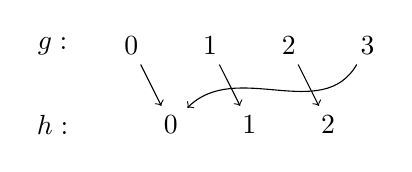
\begin{tikzpicture}
        \node at(-1,0){$g :$};
        \node(0)at(0,0){$0$};
        \node(1)at(1,0){$1$};
        \node(2)at(2,0){$2$};
        \node(3)at(3,0){$3$};
        \node at(-1,-1){$h :$};
        \node(00)at(.5,-1){$0$};
        \node(11)at(1.5,-1){$1$};
        \node(22)at(2.5,-1){$2$};
        \draw[->](0)--(00);
        \draw[->](1)--(11);
        \draw[->](2)--(22);
        \draw(3)edge[->,out=-120,in=45]node{}(00);
    \end{tikzpicture}
\end{center}
Il y a ainsi deux manières de générer $0$ par $h$ (probabilité de $\frac{1}{2}$)
alors qu'il n'y en a qu'une seule pour $1$ et $2$ (probabilités resp.
de $\frac{1}{4}$).
\bigskip

Ceci montre que le générateur aléatoire $h$ \alert{perd la propriété d'uniformité}.
\end{frame}

%%%%%%%%%%%%%%%%%%%%%%%%%%%%%%%%%%%%%%%%%%%%%%%%%%%%%%%%%%%%%%%%%%%%%%%%
\begin{frame}[fragile]
\frametitle{Mesure de la non uniformité de la réduction}
Soient $g$ un générateur aléatoire uniforme d'ordre $n$ et $h$ la
réduction de $g$ à l'ordre $k$, où $k \leq n$.
\medskip

Notons $\mathrm{gen}_h(i)$ le nombre de manières de générer l'entier
$i \leq k - 1$ par $h$. Alors, on voit facilement que
\begin{equation*}
    \mathrm{gen}_h(i) =
    \begin{cases}
        \lfloor \frac{n}{k} \rfloor + 1 &
            \mbox{si } i \in \{0, \dots, (n \mod k) -1\} \\
        \lfloor \frac{n}{k} \rfloor &
            \mbox{sinon}.
    \end{cases}
\end{equation*}

La probabilité $\mathbb{P}_h(i)$ de générer l'entier $i \leq k - 1$ par
$h$ vérifie
\begin{equation*}
    \mathbb{P}_h(i) = \frac{\mathrm{gen}_h(i)}{n}.
\end{equation*}

Les entiers $i$ de l'ensemble $\{0, \dots, k - 1\}$ ont ainsi des
probabilités différentes d'être générés. Ils se divisent en deux classes~:
\begin{enumerate}
    \item {\bf les petits}, de $0$ à $(n \mod k) - 1$, avec une probabilité
    plus grande~;
    \item {\bf les grands}, de $(n \mod k)$ à $k - 1$, avec une probabilité
    plus petite.
\end{enumerate}
\end{frame}

%%%%%%%%%%%%%%%%%%%%%%%%%%%%%%%%%%%%%%%%%%%%%%%%%%%%%%%%%%%%%%%%%%%%%%%%
\begin{frame}[fragile]
\frametitle{Mesure de la non uniformité de la réduction}
Comparons numériquement les probabilités de génération des petits et des
grands nombres pour différentes valeurs de $n$ et de $k$~:
\begin{center}
    \footnotesize
    \begin{tabular}{c|c||c|c|c}
        $n$ & $k$ & Prob. des petits & Prob. des grands & Rapport \\ \hline \hline
        $4$ & $3$ & $0.5$ & $0.25$ & $2$ \\
        $400$ & $300$ & $0.005$ & $0.0025$ & $2$ \\
        $400$ & $200$ & $0.005$ & $0.005$ & $1$ \\
        $400$ & $101$ & $0.01$ & $0.0075$ & $\simeq1.3333$ \\
        $400$ & $99$ & $0.0125$ & $0.01$ & $1.25$ \\
        $500$ & $99$ & $0.012$ & $0.01$ & $1.2$ \\
        $5000$ & $99$ & $0.0102$ & $0.01$ & $1.02$ \\
        $50000$ & $99$ & $0.01012$ & $0.0101$ & $\simeq1.00198$
    \end{tabular}
\end{center}

On observe que plus $k$ est {\bf petit} par rapport à $n$, plus $h$ se
rapproche d'un générateur {\bf uniforme}. Lorsque $k$ est un diviseur
de $n$, l'uniformité est immédiate.
\medskip

En pratique, la réduction est considérée comme préservant l'uniformité,
à condition de partir d'un générateur aléatoire d'entiers uniforme $g$
d'ordre le  plus grand possible.
\end{frame}

%%%%%%%%%%%%%%%%%%%%%%%%%%%%%%%%%%%%%%%%%%%%%%%%%%%%%%%%%%%%%%%%%%%%%%%%
%%%%%%%%%%%%%%%%%%%%%%%%%%%%%%%%%%%%%%%%%%%%%%%%%%%%%%%%%%%%%%%%%%%%%%%%
\subsection{Nombres pseudo-aléatoires}

%%%%%%%%%%%%%%%%%%%%%%%%%%%%%%%%%%%%%%%%%%%%%%%%%%%%%%%%%%%%%%%%%%%%%%%%
\begin{frame}[fragile]\frametitle{Machines et aléatoire}
Un ordinateur est par essence une \alert{machine déterministe}~: le
résultat d'un programme est toujours le même s'il est exécuté deux fois
dans les mêmes conditions.
\bigskip

Il est ainsi impossible d'écrire un programme qui implante un générateur
aléatoire d'entiers.
\bigskip

La seule chose qu'il est possible de faire est de programmer une fonction
qui {\bf semble} le plus possible se comporter comme un générateur aléatoire.
On parle alors de \alert{générateur pseudo-aléatoire}.
\bigskip

Les entiers qu'un générateur pseudo-aléatoire génère lorsqu'on l'appelle
plusieurs fois de suite forme une suite. On appelle cette suite une
suite d'\alert{entiers pseudo-aléatoires}.
\end{frame}

%%%%%%%%%%%%%%%%%%%%%%%%%%%%%%%%%%%%%%%%%%%%%%%%%%%%%%%%%%%%%%%%%%%%%%%%
\begin{frame}[fragile]\frametitle{Principe de fonctionnement}
Un générateur pseudo-aléatoire $g$ d'ordre $n$ fonctionne de la
manière suivante~:
\smallskip

\begin{itemize}
    \item il dispose d'une \alert{graine} $g_1, g_2, \dots, g_\ell$,
    qui est une suite d'entiers~;
    \smallskip

    \item lorsqu'on l'appelle pour la $r\ieme$ fois, il renvoie un
    entier $g_{\ell + r}$ calculé à partir des entiers
    $g_1, \dots, g_\ell, \dots, g_{\ell + r - 1}$ précédemment calculés,
    selon une \alert{règle} spécifiée.
\end{itemize}
\medskip

Ainsi, $g$ produit une suite d'entiers
\begin{equation*}
    g_{\ell + 1}, g_{\ell + 2}, g_{\ell + 3}, \dots
\end{equation*}
à partir de la graine dans laquelle figurent les {\bf données initiales}
et de la règle qui explique comment générer le {\bf prochain entier} de
la suite en se basant sur les {\bf entiers précédemment générés}.
\end{frame}

%%%%%%%%%%%%%%%%%%%%%%%%%%%%%%%%%%%%%%%%%%%%%%%%%%%%%%%%%%%%%%%%%%%%%%%%
\begin{frame}[fragile]\frametitle{Qualités d'un générateur pseudo-aléatoire}
Un bon générateur pseudo-aléatoire produit une suite d'entiers qui
semble aléatoire.
\medskip

Il est possible de mesurer la qualité d'un générateur aléatoire conformément
à plusieurs critères~:
\smallskip

\begin{enumerate}
    \item {\bf uniformité} de la génération~;
    \smallskip

    \item ses {\bf périodes} (longueurs des cycles de génération)~;
    \smallskip

    \item {\bf sensibilité à la graine} (existence de mauvaises graines)~;
    \smallskip

    \item {\bf corrélation} entre un entier engendré et les précédents~;
    \smallskip

    \item {\bf analyse de la distribution} en plusieurs dimensions.
\end{enumerate}
\end{frame}

%%%%%%%%%%%%%%%%%%%%%%%%%%%%%%%%%%%%%%%%%%%%%%%%%%%%%%%%%%%%%%%%%%%%%%%%
\begin{frame}[fragile]\frametitle{Méthode du carré médian}
Le générateur pseudo-aléatoire $g$ utilisant la
\alert{méthode du carré médian} fonctionne de la manière suivante.
\medskip

La graine de ce générateur est un entier compris entre $0$ et $9999$.
Si $g_{i - 1}$ est l'entier précédemment généré (ou bien la graine), le
prochain entier généré est
\begin{equation*}
    g_i := \left(\left\lfloor \frac{g_{i - 1}}{10} \right\rfloor \mod 100\right)^2.
\end{equation*}

On obtient p.ex. les suites
\begin{center} \footnotesize
    \begin{tabular}{c|c}
        Graine & Suite \\ \hline
        1234 & 529, 2704, 4900, 8100, 100, 100, ... \\
        3733 & 5329, 1024, 4, 0, 0, ... \\
        9999 & 9801, 6400, 1600, 3600, 3600, ...
    \end{tabular}
\end{center}
\medskip

C'est un {\bf mauvais générateur pseudo-aléatoire}. Les périodes sont
bien trop courtes et il y a des mauvaises graines (comme $0$).
\end{frame}

%%%%%%%%%%%%%%%%%%%%%%%%%%%%%%%%%%%%%%%%%%%%%%%%%%%%%%%%%%%%%%%%%%%%%%%%
\begin{frame}[fragile]\frametitle{Méthode additive}
Le générateur pseudo-aléatoire $g$ utilisant la \alert{méthode additive}
fonctionne de la manière suivante.
\medskip

On se fixe un ordre $n \geq 1$. La graine de ce générateur est
un triplet $(g_1, g_2, g_3)$ d'entiers compris entre $0$ et $n - 1$.
La génération de $g_i$ dépend des trois entiers précédemment
générés $g_{i - 1}$, $g_{i - 2}$ et $g_{i - 3}$. Il est défini par
\begin{equation*}
    g_i := (g_{i - 1} + g_{i - 2} + g_{i - 3}) \mod n.
\end{equation*}

On obtient p.ex. les suites
\begin{center} \scriptsize
    \begin{tabular}{c|c|c}
        $n$ & Graine & Suite \\ \hline
        211 & $(1, 1, 1)$ & 3, 5, 9, 17, 31, 57, 105, 193, 144, 20, 146,
            99, 54, 88, 30, 172, 79 \\
        3099 & $(1, 1, 1)$ & 3, 5, 9, 17, 31, 57, 105, 193, 355, 653, 1201,
            2209, 964, 1275, 1349 \\
        1347 & $(600, 31, 1)$ & 632, 1263, 1148, 349, 66, 216, 631, 913,
            413, 610, 589, 265, 117
    \end{tabular}
\end{center}
\medskip

Ce générateur pseudo-aléatoire est bien meilleur que le précédent mais
échoue à de nombreux tests statistiques.
\end{frame}

%%%%%%%%%%%%%%%%%%%%%%%%%%%%%%%%%%%%%%%%%%%%%%%%%%%%%%%%%%%%%%%%%%%%%%%%
\begin{frame}[fragile]\frametitle{Générateurs congruentiels linéaires}
Un générateur pseudo-aléatoire $g$ \alert{congruentiel linéaire} fonctionne
de la manière suivante.
\medskip

On se fixe un ordre $n \geq 1$ ainsi que deux entiers positifs $a$ et $b$.
La graine de ce générateur est un entier compris entre $0$ et $n - 1$.
La génération de $g_i$ dépend de l'entier précédemment généré $g_{i - 1}$
et est défini par
\begin{equation*}
    g_i := (a \times g_{i - 1} + b) \mod n.
\end{equation*}

On obtient p.ex. les suites
\begin{center} \scriptsize
    \begin{tabular}{c|c|c|c|c}
        $n$ & $a$ & $b$ & Graine & Suite \\ \hline
        128 & 3 & 1 & 1 & 4, 13, 40, 121, 108, 69, 80, 113, 84, 125,
            120, 105, 60 \\
        128 & 7 & 1 & 1 & 8, 57, 16, 113, 24, 41, 32, 97, 40, 25,
        48, 81, 56, 9, 64 \\
        $2^{32}$ & 1664525 & 1013904223 & 1 &
            1015568748, 1586005467, 2165703038, 3027450565 \\
    \end{tabular}
\end{center}
\medskip

Sous réserve de choisir des bons paramètres $n$, $a$ et $b$, ce
générateur pseudo-aléatoire est plutôt bon. Il est très utilisé en
pratique.
\end{frame}

%%%%%%%%%%%%%%%%%%%%%%%%%%%%%%%%%%%%%%%%%%%%%%%%%%%%%%%%%%%%%%%%%%%%%%%%
%%%%%%%%%%%%%%%%%%%%%%%%%%%%%%%%%%%%%%%%%%%%%%%%%%%%%%%%%%%%%%%%%%%%%%%%
\subsection{Utilisation et implantation}

%%%%%%%%%%%%%%%%%%%%%%%%%%%%%%%%%%%%%%%%%%%%%%%%%%%%%%%%%%%%%%%%%%%%%%%%
\begin{frame}[fragile]\frametitle{Les fonctions {\tt rand} et {\tt srand}}
La fonction
\begin{center} \Code{int rand();} \end{center}
du module \Code{stdlib} implante un générateur pseudo-aléatoire d'ordre
\Code{RAND\_MAX + 1}. C'est un générateur congruentiel linéaire. À chaque
appel, il renvoie le prochain entier de la suite.
\bigskip
\bigskip

La graine de ce générateur peut-être affectée par la fonction
\begin{center} \Code{void srand(unsigned int g1);} \end{center}
Par défaut, la graine du générateur est \Code{1}.
\end{frame}

%%%%%%%%%%%%%%%%%%%%%%%%%%%%%%%%%%%%%%%%%%%%%%%%%%%%%%%%%%%%%%%%%%%%%%%%
\begin{frame}[fragile]
\frametitle{Modèle d'utilisation de {\tt rand} et de {\tt srand}}
\begin{multicols}{2}
Tout projet qui utilise la fonction \Code{rand} doit avoir une fonction
principale \Code{main} de la forme ci-contre.
\smallskip

L'appel à \Code{srand} doit être fait le plus tôt possible.

\begin{center}
\begin{minipage}[c]{.4\textwidth}
\begin{lstlisting}[frame=single,numbers=none,basicstyle=\scriptsize\tt]
/* Main.c */
...
#include <stdlib.h>
#include <time.h>
...
int main() {
    ...
    srand(time(NULL));
    ...
}
\end{lstlisting}
\end{minipage}
\end{center}
\end{multicols}

La fonction \Code{time\_t time (time\_t* timer);}
du module \Code{time}, lorsque appelée avec l'argument \Code{NULL}
renvoie le temps écoulé en secondes depuis le 1\ier{} janvier 1970 à
minuit, UTC.
\medskip

Considérer cette valeur est donc un bon moyen d'initialiser la graine
du générateur.
\medskip

{\bf Attention} ({\em point très important})~: il est totalement erroné
d'initialiser dans un même projet deux fois la graine. Le seul appel à
\Code{srand} doit figurer dans \Code{main} et nulle part ailleurs.
\end{frame}

%%%%%%%%%%%%%%%%%%%%%%%%%%%%%%%%%%%%%%%%%%%%%%%%%%%%%%%%%%%%%%%%%%%%%%%%
\begin{frame}[fragile]\frametitle{Implantation avec variable globale}
Une implantation possible des fonctions \Code{rand} et \Code{srand}
s'appuie sur une {\bf variable globale} pour mémoriser la dernière valeur
générée.
\medskip

\begin{center}
\begin{minipage}[c]{.41\textwidth}
\begin{lstlisting}[frame=single,numbers=none,basicstyle=\scriptsize\tt]
/* RandPerso.h */
#ifndef __RAND_PERSO__
#define __RAND_PERSO__

    #define RAND_PERSO_ORDRE 32767
    #define RAND_PERSO_A 1024
    #define RAND_PERSO_B 1
    #define RAND_PERSO_GRAINE 1

    int rand_perso();
    void srand_perso(int graine);

#endif
\end{lstlisting}
\end{minipage}
\quad
\begin{minipage}[c]{.45\textwidth}
\begin{lstlisting}[frame=single,numbers=none,basicstyle=\scriptsize\tt]
/* RandPerso.c */
#include "RandPerso.h"

unsigned int valeur_rand =
    RAND_PERSO_GRAINE;

int rand_perso() {
    valeur_rand =
        (valeur_rand * RAND_PERSO_A
            + RAND_PERSO_B)
        % RAND_PERSO_ORDRE;
    return valeur_rand;
}

void srand_perso(int graine) {
    valeur_rand = graine;
}
\end{lstlisting}
\end{minipage}
\end{center}
\end{frame}

%%%%%%%%%%%%%%%%%%%%%%%%%%%%%%%%%%%%%%%%%%%%%%%%%%%%%%%%%%%%%%%%%%%%%%%%
\begin{frame}[fragile]\frametitle{Implantation avec variable statique}
Dans cette implantation, on utilise une {\bf variable statique} pour
mémoriser la dernière valeur générée.

\begin{center}
\begin{minipage}[c]{.41\textwidth}
\begin{lstlisting}[frame=single,numbers=none,basicstyle=\scriptsize\tt]
/* RandPerso.h */
#ifndef __RAND_PERSO__
#define __RAND_PERSO__

    #define RAND_PERSO_ORDRE 32767
    #define RAND_PERSO_A 1024
    #define RAND_PERSO_B 1
    #define RAND_PERSO_GRAINE 1

    int rand_perso();

#endif
\end{lstlisting}
\end{minipage}
\quad
\begin{minipage}[c]{.45\textwidth}
\begin{lstlisting}[frame=single,numbers=none,basicstyle=\scriptsize\tt]
/* RandPerso.c */
#include "RandPerso.h"

#include <time.h>

int rand_perso() {
    static int premier_appel = 1;
    static unsigned int valeur_rand;
    if (premier_appel) {
        valeur_rand = time(NULL);
        premier_appel = 0;
    }
    valeur_rand =
        (valeur_rand * RAND_PERSO_A
            + RAND_PERSO_B)
        % RAND_PERSO_ORDRE;
    return valeur_rand;
}
\end{lstlisting}
\end{minipage}
\end{center}

\begin{small}
L'initialisation ne se fait qu'au 1\ier{} appel et l'utilisateur n'a
pas à la faire explicitement. Avec cette méthode, il n'est pas possible
de fixer la graine.
\end{small}
\end{frame}

%%%%%%%%%%%%%%%%%%%%%%%%%%%%%%%%%%%%%%%%%%%%%%%%%%%%%%%%%%%%%%%%%%%%%%%%
\begin{frame}[fragile]\frametitle{Retrouver le déterminisme}
Pour pouvoir reproduire les résultats fournis par un programme utilisant
la fonction \Code{rand}, il est nécessaire de proposer un
\alert{mode de fonctionnement déterministe} dans lequel la graine a été
fixée.
\medskip

Pour cela, on met en place dans le module principal d'un projet et dans sa
fonction \Code{main} le mécanisme suivant~:
\begin{multicols}{2}
\begin{center}
\begin{minipage}[c]{.35\textwidth}
\begin{lstlisting}[frame=single,numbers=none,basicstyle=\scriptsize\tt]
/* Main.c */
...
#define DETERMINISTE
...
int main() {
    ...
#ifdef DETERMINISTE
    srand(0);
#else
    srand(time(NULL));
#endif
    ...
}
\end{lstlisting}
\end{minipage}
\end{center}
De cette manière, on peut imposer un comportement déterministe
({\bf reproductible}) à l'exécution du projet en gardant la définition
de la macro \Code{DETERMINISTE}.
\smallskip

Pour éviter ce comportement, il suffit de commenter cette macro-définition.
\end{multicols}

\begin{footnotesize}
Meilleure solution~: utiliser l'option \Code{-D} de \Code{gcc}. Il
suffit de supprimer la ligne \Code{\#define DETERMINISTE} et de compiler
avec \Code{-DDETERMINISTE} pour définir la macro en question.
\end{footnotesize}
\end{frame}
